Összefoglaló az első mérési fázis eredményeiről. A hét ismert modell tanítás nélküli eredeti élsúlyokkal történő vizsgálata történt meg a saját ImageNet1k osztályozású adathalmazomon ami összesen 180750 képet tartalmaz 114 imagenet osztályba sorolva ahol nincs 300 képnél kisebb kategória Train, Val, Test halmazokra osztva 80, 10, 10 arányban. Így a Test halmaz 18172 képet tartalmaz szintén 114 kategóriára osztva. Ezen történt a hét ismert modell első fázisú tesztelése saját tanítás nélküli eredeti ImageNet1k-n előtanított súlyokkal. Nézzük most ennek a vizsgáltnak az eredményeit.


\subsection{Összefoglaló táblázat az első fázis mért értékeiről}
\begin{center}
    \begin{longtable}{lllllll}
    \caption{Modellek összefoglaló értékei tanítás nélkül}\label{tab:phase1_summary_table}\\
    \toprule
    Modell & Top-1 Acc. & Top-5 Acc. & Precision & Recall & F1-score & Idő(s) \\
    \midrule
    \endfirsthead
    \toprule
    Modell & Top-1 & Top-5 & Precision & Recall & F1-score & Idő(s) \\
    \midrule
    \endhead
    ConvNeXt-Tiny & 0.5048 & 0.8471 & 0.4917 & 0.4369 & 0.4194 & 38.40 \\
    ViT-B/16 & 0.5308 & 0.8582 & 0.4629 & 0.4419 & 0.4307 & 92.13 \\
    EfficientNet-B0 & 0.4802 & 0.8217 & 0.4137 & 0.4039 & 0.3829 & 28.89 \\
    ResNet50 & 0.4698 & 0.7962 & 0.3934 & 0.3797 & 0.3592 & 25.21 \\
    DenseNet121 & 0.4498 & 0.7806 & 0.3874 & 0.3611 & 0.3408 & 25.15 \\
    Inception-v3 & 0.4763 & 0.8008 & 0.3833 & 0.3896 & 0.3683 & 38.06 \\
    NASNet & 0.2820 & 0.5408 & 0.3204 & 0.2799 & 0.2696 & 275.30 \\
    \bottomrule
    \end{longtable}
    \end{center}

\subsection{Top 1 és Top 5 pontosságok összehasonlítása modellenként tanítás nélkül.}
    \begin{figure}[H]
        \centering
        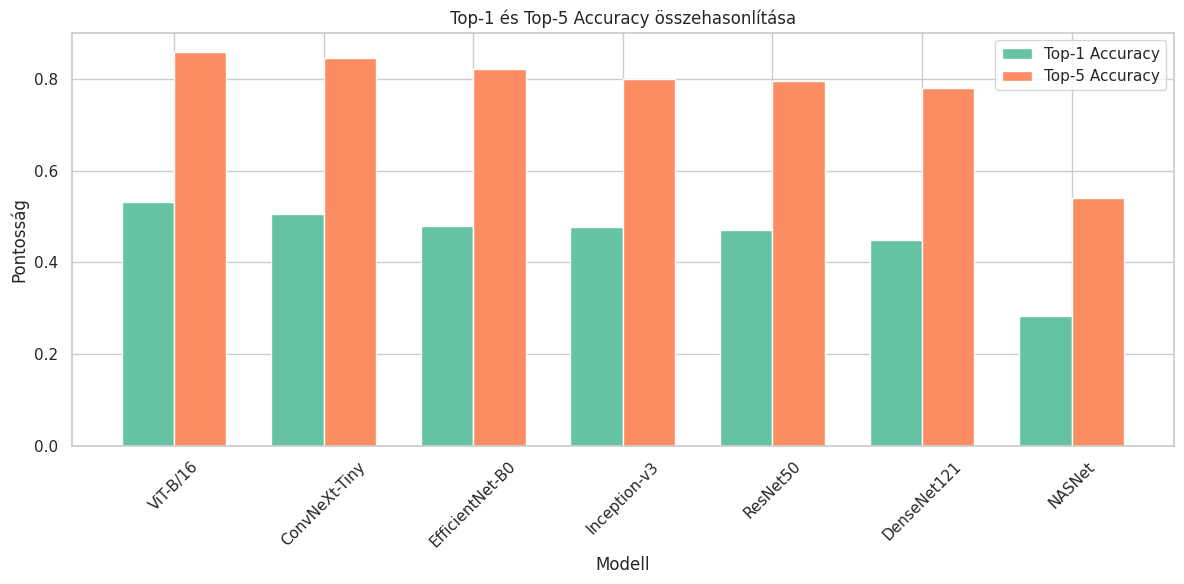
\includegraphics[width=1.0\textwidth]{images/phase01/summary01.png}
        \caption{Top 1 és Top 5 pontosságok összehasonlítása modellenként tanítás nélkül.}
        \label{fig:phase01_summary01}
    \end{figure}

\subsection{Precision, Recall, F1-score összehasonlítása modellenként tanítás nélkül.}
    \begin{figure}[H]
        \centering
        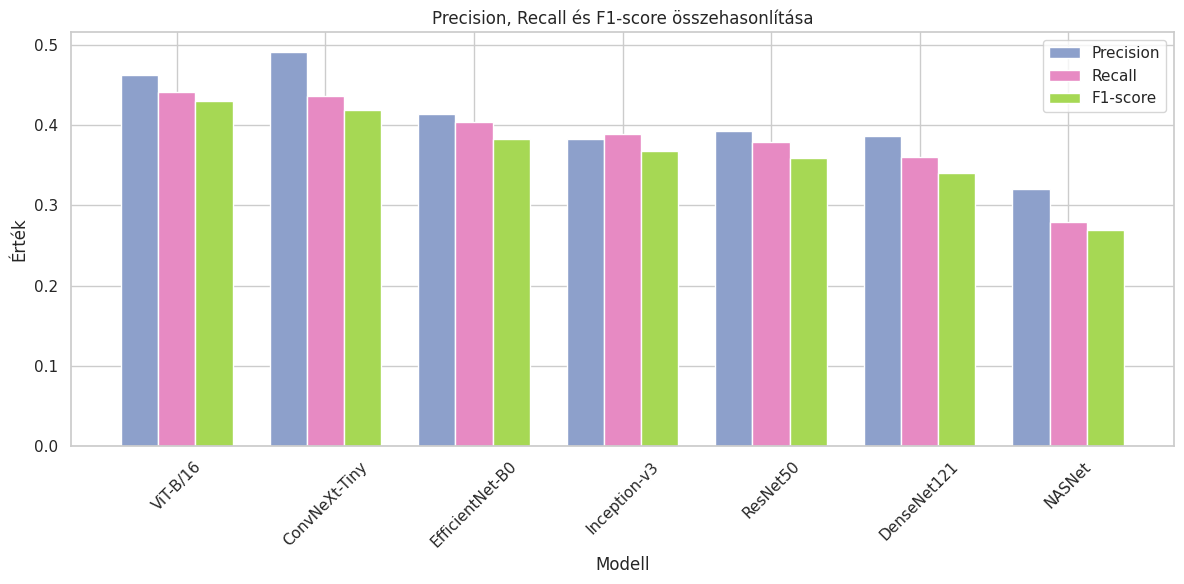
\includegraphics[width=1.0\textwidth]{images/phase01/summary02.png}
        \caption{Precision, Recall, F1-score összehasonlítása modellenként tanítás nélkül.}
        \label{fig:phase01_summary02}
    \end{figure}

\subsection{Teszt lefutási idejének összehasonlítása modellenként tanítás nélkül.}
    \begin{figure}[H]
        \centering
        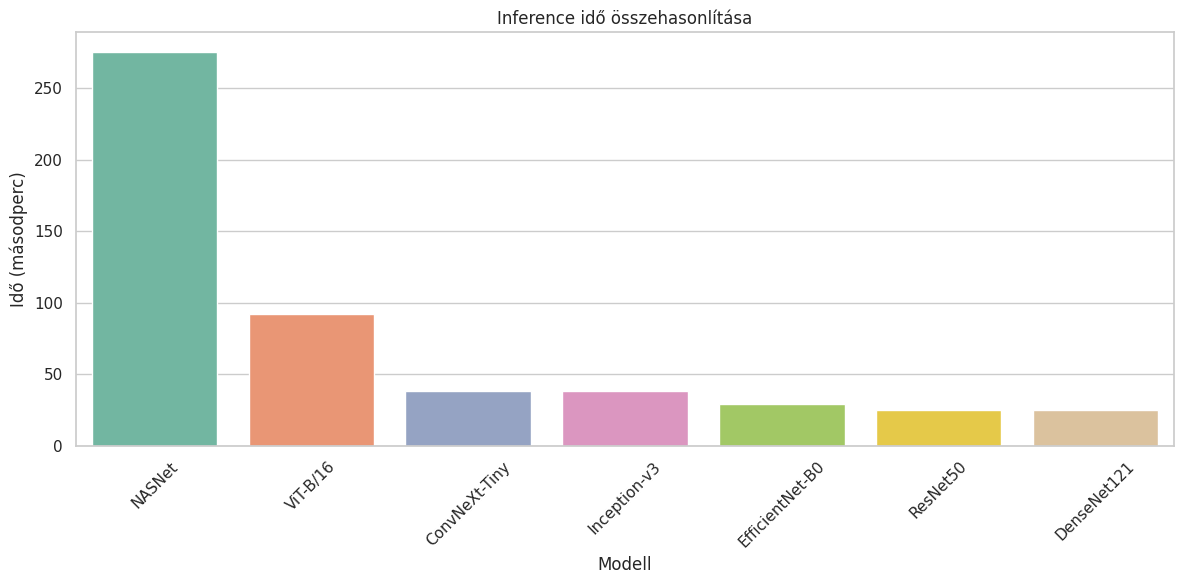
\includegraphics[width=1.0\textwidth]{images/phase01/summary03.png}
        \caption{Teszt lefutási idejének összehasonlítása modellenként tanítás nélkül.}
        \label{fig:phase01_summary03}
    \end{figure}

\subsection{Az első fázis rövid szöveges értékelése}
Az első mérési fázis során hét különböző, előre betanított modellt teszteltem a saját sb-photothemes-imagenet114 adatbázis 18000 képből álló, 114 kategóriát tartalmazó teszthalmazán. A modelleket itt az első fázisban tanítás nélkül, a gyári súlyokkal értékeltem.

Pontosság tekintetében a ViT-B/16 modell érte el a legjobb Top-1 (53,08\%) és Top-5 (85,82\%) pontosságot, szorosan követi a ConvNeXt-Tiny és az EfficientNet-B0. Ezek az eredmények azt mutatják, hogy a transformer-alapú és modern CNN architektúrák jobban teljesítenek a hagyományosabb modelleknél, mint például a ResNet50 vagy a DenseNet121. A NASNet jelentősen alacsonyabb pontosságot ért el, ami arra utalhat, hogy nem optimalizált az adott teszthalmazra.

Precision, Recall és F1-score mutatók alapján a ViT-B/16 és a ConvNeXt-Tiny modellek kiemelkednek, ami megerősíti a pontossági eredményeket. Ezek a modellek nemcsak pontosak, hanem megbízhatóak is a kategóriák felismerésében.

Inference idő szempontjából a DenseNet121 és a ResNet50 modellek a leggyorsabbak (~25 másodperc), míg a NASNet jelentősen lassabb (275,30 másodperc), ami korlátozhatja a gyakorlati alkalmazhatóságát, különösen valós idejű rendszerekben.

Összegzésként, a ViT-B/16 és a ConvNeXt-Tiny modellek kínálják a legjobb kompromisszumot a pontosság és a teljesítmény között, bár a ViT-B/16 jelentősen hosszabb inference idővel rendelkezik. A DenseNet121 és a ResNet50 gyorsabbak, de alacsonyabb pontosságot nyújtanak. A NASNet alacsony pontossága és hosszú inference ideje miatt kevésbé ajánlott az adott feladatra.